\documentclass{article}
\usepackage{graphicx}
\usepackage{subfigure}

\begin{document}

\section{Pneumatic Diagram}
\subsection{Inner Circuit}
\begin{figure}[h]
\centering
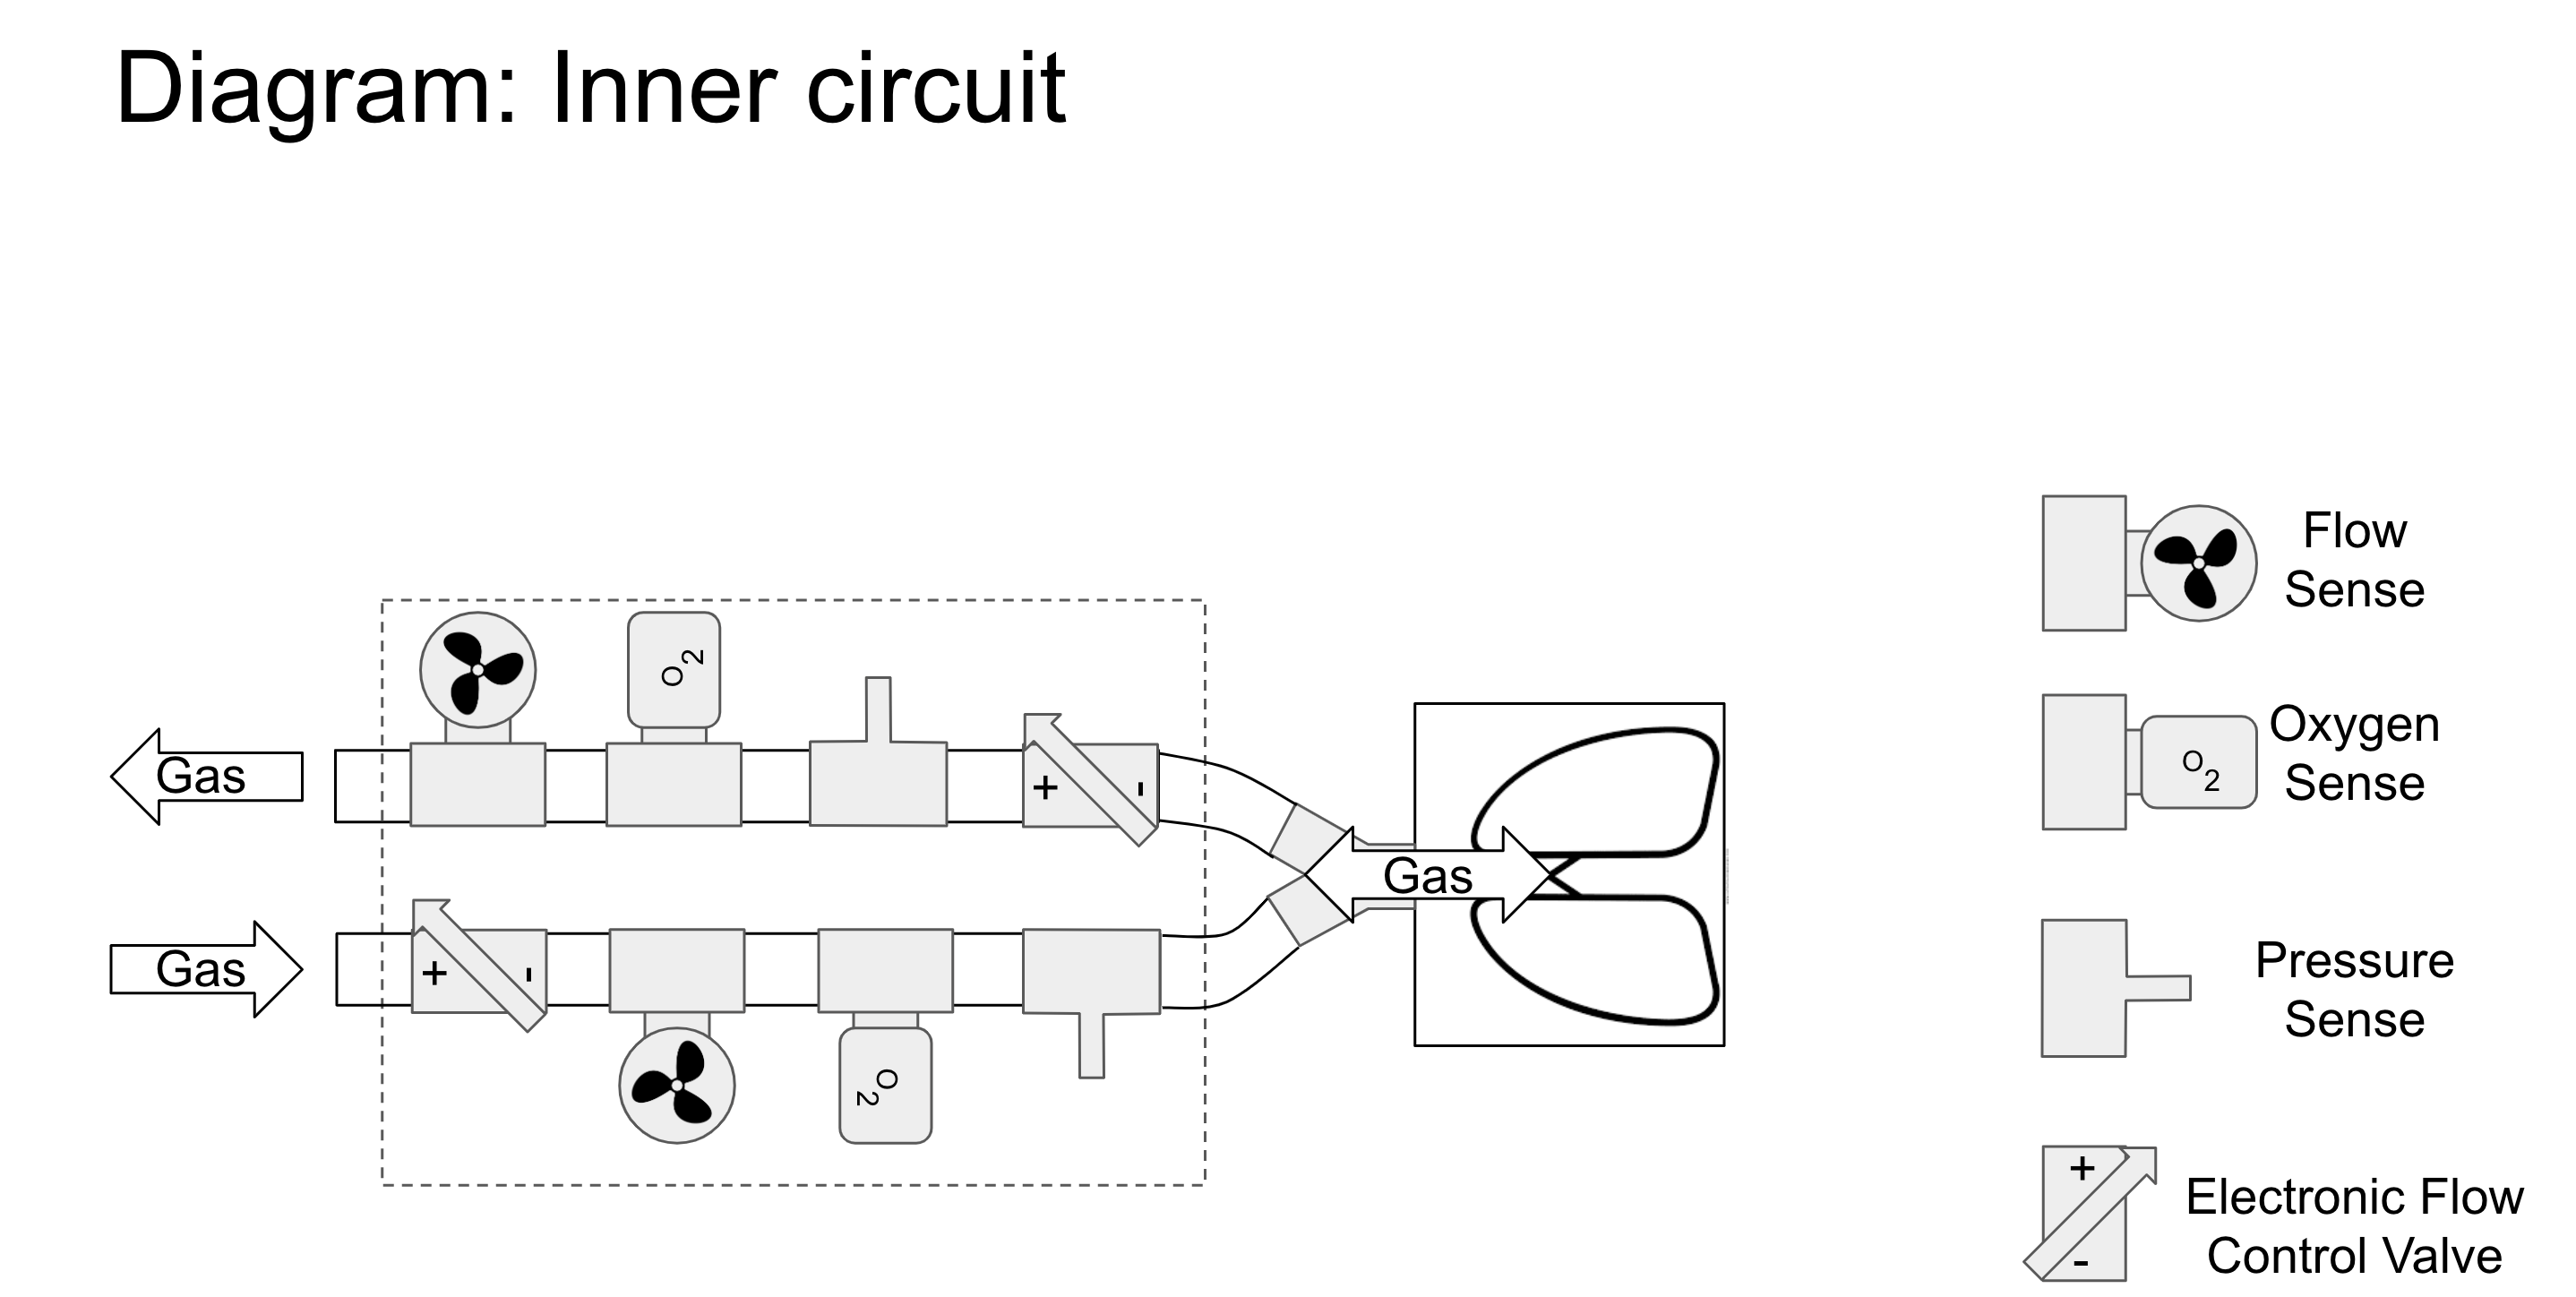
\includegraphics[scale=0.25]{pneumatic-diagram-inner.png}
\end{figure}

The two flow control valves will both be one-way. The lower tube is the inhalation tube and the upper tube is the exhalation tube.

\subsection{Outer Circuit}
\begin{figure}[h]
\centering
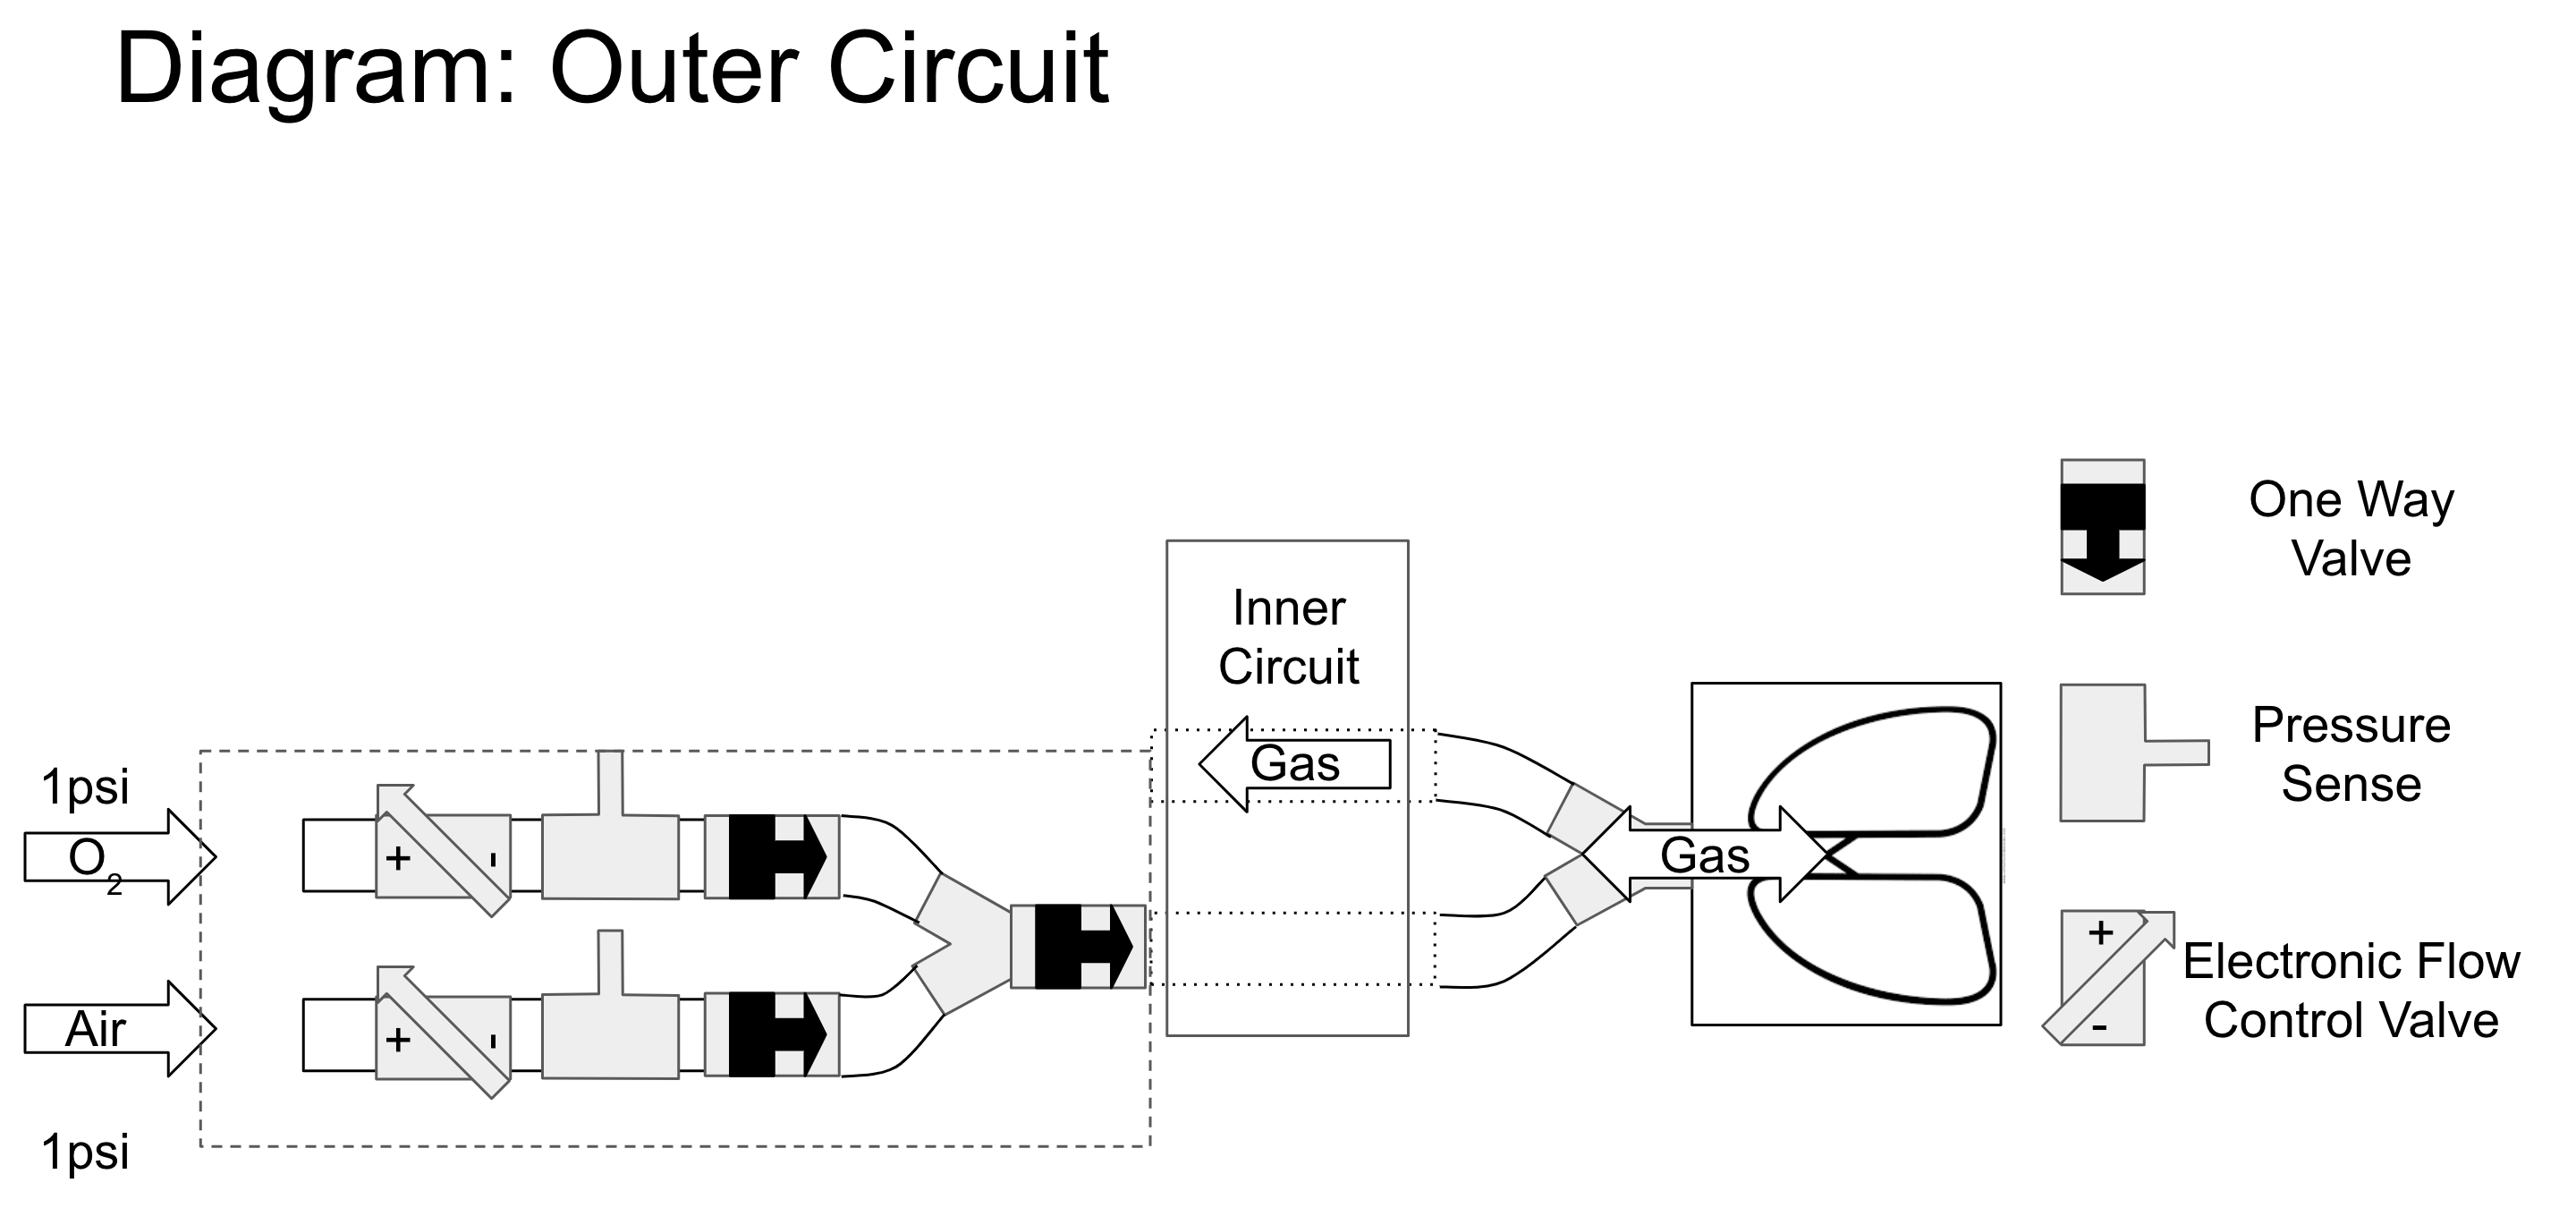
\includegraphics[scale=0.25]{pneumatic-diagram-outer.png}
\end{figure}

\newpage

\section{Inhalation}
\subsection{Control Circuit}
\begin{figure}[h]
\centering
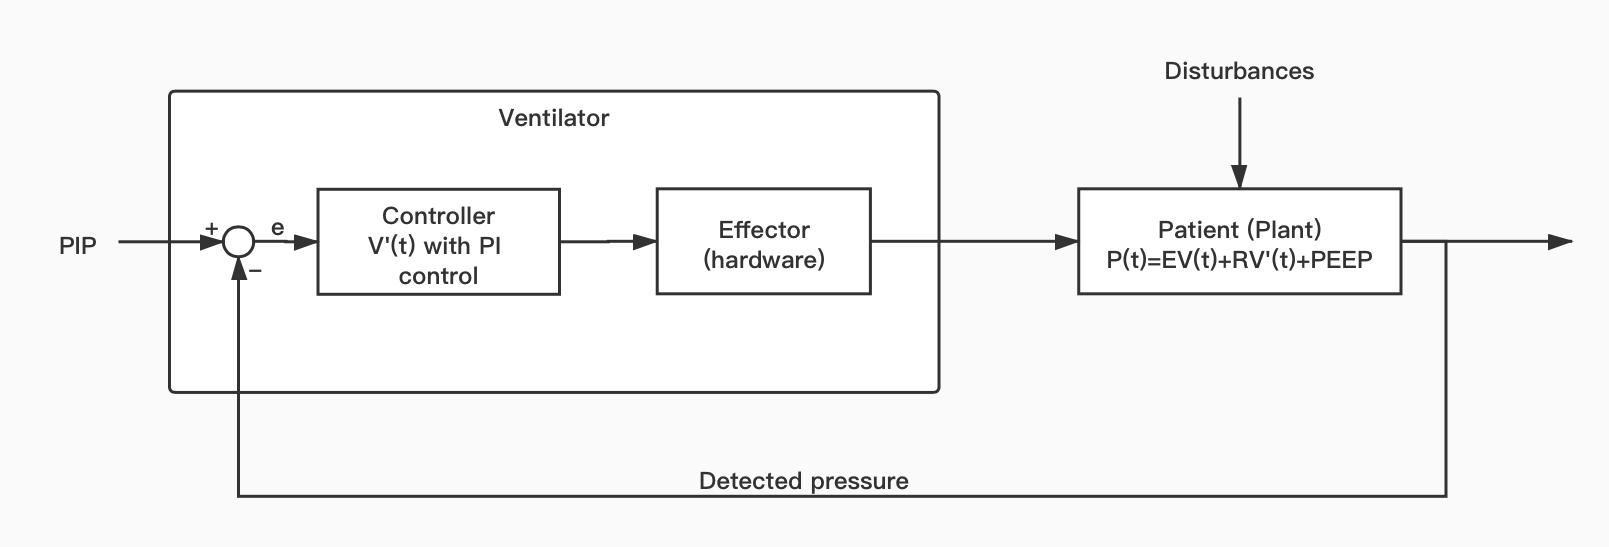
\includegraphics[scale=0.23]{control-circuit.jpg}
\end{figure}

The control circuit for inhalation. The input $PIP$ (Peak Inspiratory Pressure) is the expected level of pressure to reach. Error $e$ is the difference between actual pressure $P(t)$ measured by the sensor and $PIP$. $V(t)$ is the volume of air in patient's alveoli and $V'(t)$ would represent the flow speed of the injected gas. PI control is used in the circuit. The formula for the controller is :
$$V'(t)=K_pe+K_i\int _0^tedt$$
For the plant, the formula
$$P(t)=EV(t)+RV'(t)+PEEP$$
is the equation of motion, which shows a mathematical relation between the physical properties in the patient's lung. $E$ represents the elastance (inverse of the compliance) of the patient's lung and $R$ represents the airway resistance. $PEEP$ (Positive End Expiratory Pressure) is the remaining positive pressure in the patient's lung after exhalation. It is usually set as positive manually to prevent atelectasis.

\newpage

\subsection{Flow Diagram}
\begin{figure}[h]
\centering
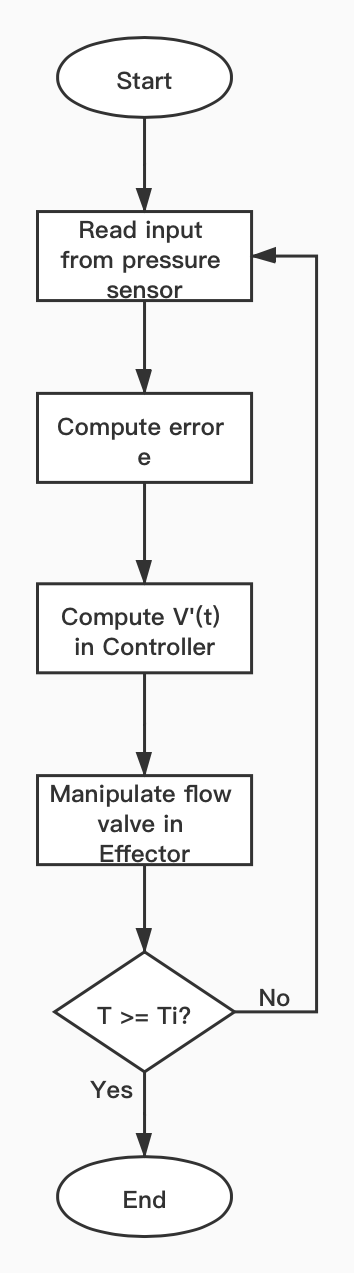
\includegraphics[scale=0.3]{flow-diagram.jpg}
\end{figure}

The flow diagram for a single inhalation. It can be triggered either by the machine or by patient. When the time $T$ has exceed the preset inspiratory time $Ti$, the inhalation would end and the exhalation would begin.

\newpage

\subsection{Transfer Function}
\begin{figure}[h]
\centering
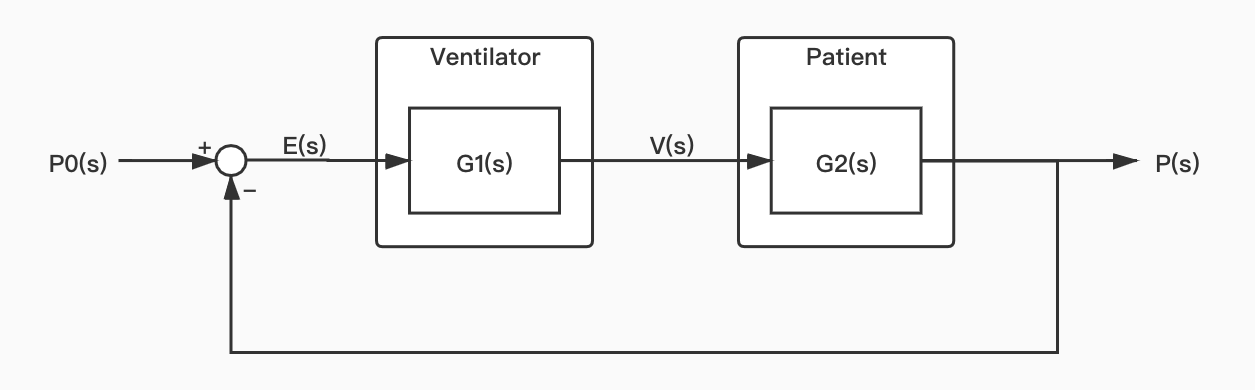
\includegraphics[scale=0.3]{block-diagram.jpg}
\end{figure}

$E(s)$, $V(s)$, $P(s)$ is the Laplace transforms of the error $e(t)$, volume $v(t)$ and the pressure $p(t)$. The input $P_{0}(s)$ is the Laplace transform of $p_{0}$, while $p_{0}$ is $PIP-PEEP$. $PEEP$ is subtracted from $PIP$ so that the zero initial condition of the system can be satisfied ($p(0)=0$). $G_1(s)$ is the transfer function of the ventilator and $G_2(s)$ is the transfer function of the patient.

For ventilator:
$$v'(t)=K_pe+K_i\int _0^tedt$$
Do Laplace transform on both sides:
$$sV(s)=K_pE(s)+\frac{K_i}{s}E(s)$$
$$G_1(s)=\frac{V(s)}{E(s)}=\frac{K_p}{s}+\frac{K_i}{s^2}$$

For patient:
$$p(t)=Ev(t)+Rv'(t)$$
Do Laplace transform on both sides:
$$P(s)=EV(s)+RsV(s)$$
$$G_2(s)=\frac{P(s)}{V(s)}=E+Rs$$
$$G(s)=\frac{P(s)}{E(s)}=G_1(s)\cdot G_2(s)=(\frac{K_p}{s}+\frac{K_i}{s^2})(E+Rs)$$
$$P(s)=G(s)\cdot E(s)=G(s)\cdot (P_0(s)-P(s))$$
$$\frac{P(s)}{P_0(s)}=\frac{G(s)}{1+G(s)}$$
Therefore, the transfer function of the system is:
$$\frac{P(s)}{P_0(s)}=\frac{G(s)}{1+G(s)}=\frac{K_pRs^2+(K_pE+K_iR)s+K_iE}{(K_pR+1)s^2+(K_pE+K_iR)s+K_iE}$$

\section{Exhalation}
The exhalation process is divided into two parts: 1. Let the gas in the patient's lung goes out naturally 2. Involve a PI control to maintain the pressure on a constant level ($PEEP$). 

For the first part, simply open the exhalation valve. However, instead of completely closing the inhalation valve, a basic flow is delivered by the inhalation tube to help the gas in the lung comes out.

For the second part, when the level of pressure has approached preset level ($PEEP$), a PI control will be involved to maintain it. All of the logic here is the same as in the inhalation process. In this case, the input for the control circuit will be $PEEP$ instead of $PIP$. The flow of the control program is the same, and will also ends when it passes the preset time (determined by $Ti$ and $I:E ratio$). The transfer function is also the same, while the input $P_0(s)$ will be $0$ ($\Delta P=PEEP-PEEP=0$).

\section{Effector}
From the perspective of hardware, flow is manipulated by controlling the inhalation valve and exhalation valve. To get a positive flow, the inhalation valve will be opened accordingly and the exhalation valve will be closed. To get a negative flow, the exhalation valve will be opened accordingly and the inhalation valve will be closed. In whichever situation, we can choose the pressure sensor in the inhalation tube as the feedback signal. \textbf{(Michael: the pressure sensor in the exhalation tube seems to be redundant?)}

\section{Inhale-exhale Cycle}
The cycle will be manipulated by the preset time. The logic for patient-triggered breath will be added later but the general idea is: if a negative pressure in the lung is detected after the exhalation (pressure has reached $PEEP$) and before the inhalation, which means the patient want to start a breath spontaneously, the inhalation process will be immediately started and the cycle will be reset.

\section{Weaning Test}
For now, the idea is present the RSBI, which is an index that helps the doctor to determine when to perform the extubation, to the doctor. More details will be added.

\section{Compliance Tracking}
More details will be added later. Basic idea:
$$\frac{1}{C}=\frac{plateau-peep}{V_T}$$. The compliance will be measured every time when the pressure reached plateau pressure.

\end{document}
